\documentclass[11pt,twoside]{article}
\usepackage[toc,page,header]{appendix}
\usepackage{pdfpages}
\usepackage{color}
\usepackage{csquotes}
\usepackage{changepage}
\usepackage{fontspec}
\defaultfontfeatures{Scale=MatchLowercase}
\setmainfont[Mapping=tex-text]{Times New Roman}
\setsansfont[Mapping=tex-text]{Arial}
\setmonofont{Courier}

\usepackage{float}
%% \floatstyle{boxed}
%% \restylefloat{figure}


\usepackage{graphicx}
\usepackage{caption}
\usepackage{subcaption}

\usepackage{tikz}
\usetikzlibrary{arrows,shapes,patterns,backgrounds}
\usepackage{pgfplots}
\pgfplotsset{compat=1.9}


%% %%%<
\usepackage{verbatim}
%% \usepackage[active,tightpage]{preview}
%% \setlength\PreviewBorder{0pt}%
%% %%%>


\begin{comment}
:Title: PGFPlots examples

\end{comment}

\usepackage{xifthen}

%%%% macros %%%%

\makeatletter
\newcommand*{\centerfloat}{%
  \parindent \z@
  \leftskip \z@ \@plus 1fil \@minus \textwidth
  \rightskip\leftskip
  \parfillskip \z@skip}
\makeatother


%%%%%%%%%%%%%%%%
\title{Moments}
\author{G. A. Reynolds}
\date{\today}

%%%%%%%%%%%%%%%%%%%%%%%%%%%%%%%%%%%%%%%%%%%%%%%%%%%%%%%%%%%%%%%%
\begin{document}

\maketitle
\nocite{*}

\tableofcontents
%% \listoffigures

\section{Moments}

\begin{figure}[h!]
\centering
\begin{subfigure}[b!]{0.3\textwidth}
\centering
\begin{tikzpicture}
[c/.style={insert path={circle[radius=1pt]}}]
% [c/.style={insert path={fill=black,circle,radius=2pt}}];
\filldraw (0,0)
	-- (0,4) circle (1pt) node[label=left:$x$]{}
	-- (0,5) circle (1pt) node[label=left:$\mu$] {} ;
\draw[->] (0.5,5.8) node[above=2pt] {\textcolor{red}{$\mu-x$}}
	.. controls+(down:.5cm) and +(right:.5cm) .. (0,4.5) ;
%% \draw (-0.2,2.5) node[left,align=center] {\textcolor{red}{$\mu-x $} = deviation\\
%% as length} ;
\end{tikzpicture}
\caption{Deviation as length}
\end{subfigure}
\hspace{20pt}
%%%%%%%%%%%%%%%%
\begin{subfigure}[b!]{0.6\textwidth}
\centering
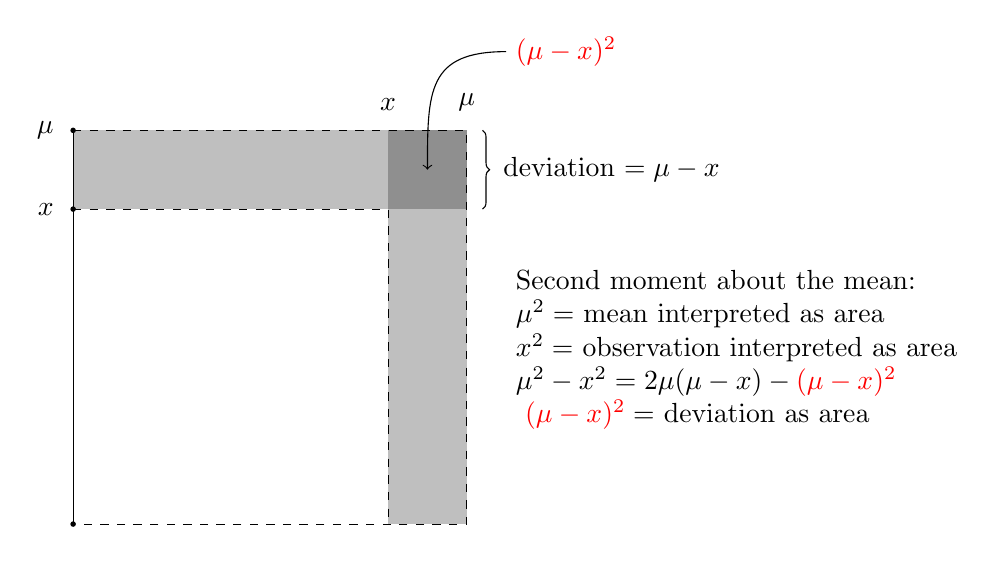
\begin{tikzpicture}
[c/.style={insert path={circle[radius=1pt]}}]
% [c/.style={insert path={fill=black,circle,radius=2pt}}];
\draw %[label distance=22pt]
	(0,0) node (origin) {}
	-- (0,5) node[label=left:$\mu$] (mean) {} ;
\draw[dashed] (0, 5)
	-- (4,5) node[label=above:$x$] {}
	-- (5,5) node[label=above:$\mu$] {}
        -- (5,0)
        -- (0,0);
\draw[dashed] (0,4) node[label={left:$x$}] (observed) {}
	-- (4,4)
        -- (4,0) ;

\draw[decorate,decoration=brace] (5.2,5) -- (5.2,4) node [midway,right=4pt] {deviation $= \mu - x$} ;

\fill[nearly transparent] (0,4) rectangle (5,5);
\fill[nearly transparent] (4,0) rectangle (5,5);

\draw (5.5,2) node[right,align=left] {Second moment about the mean:\\
$\mu^2 = $ mean interpreted as area \\
$x^2 = $ observation interpreted as area \\
$\mu^2-x^2 = 2\mu(\mu-x) - \textcolor{red}{(\mu-x)^2}$ \\
\vspace{12pt}
$\textcolor{red}{(\mu - x)^2} = $ deviation as area
} ;

\draw[->] (5.5,6) node[right] {\textcolor{red}{$(\mu-x)^2$}} .. controls+(left:1cm) and +(up:1cm) .. (4.5,4.5) ;

\fill (origin) [c] (observed) [c] (mean) [c] ;
\end{tikzpicture}
\caption{Deviation as area}
\end{subfigure}
\caption{Geometric interpretation(s) of deviation}
%Mean ($\mu$) and observation ($x$)}
\end{figure}


\begin{figure}[h!]
\centering
% Preamble: \pgfplotsset{width=7cm,compat=1.9}
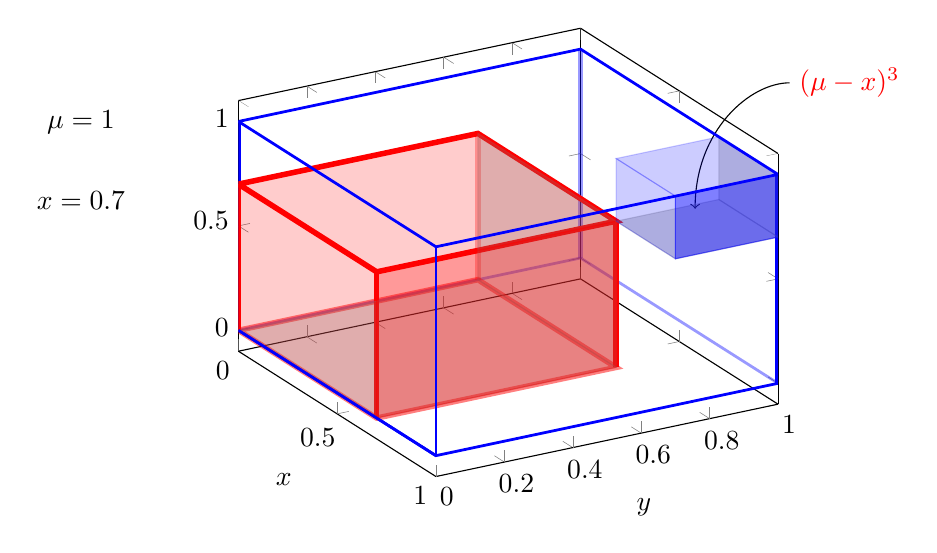
\begin{tikzpicture}

\draw (-2,4.5) node {$\mu=1$};
\draw (-2,3.5) node {$x=0.7$};

\draw[->] (7,5) node[right] {\textcolor{red}{$(\mu-x)^3$}}
	.. controls+(left:.5cm) and +(up:1cm) .. (5.8,3.4) ;

\begin{axis}[xlabel=$x$,ylabel=$y$,y domain=0:1,view={60}{30}]

%% mean = 1 outline
\addplot3[blue,line width=1pt] coordinates {(0,0,0) (1,0,0) (1,1,0)};
\addplot3[blue,opacity=.4,line width=1pt] coordinates {(1,1,0) (0,1,0)};
\addplot3[blue,opacity=.4,line width=1pt] coordinates {(0,0,0) (0,1,0)};
\addplot3[blue,opacity=.4,line width=2pt] coordinates {(0,1,0) (0,1,1)};

\addplot3[blue,line width=2pt] coordinates {(0,0,0) (0,0,1)};
\addplot3[blue,line width=2pt] coordinates {(1,1,0) (1,1,1)};


%% observed x = .7 outline
\addplot3[red,line width=2pt,opacity=.5] coordinates {(0,0,0) (.7,0,0) (.7,.7,0) (0,.7,0) (0,0,0)};
\addplot3[red,line width=2pt] coordinates {(0,0,.7) (.7,0,.7) (.7,.7,.7) (0,.7,.7) (0,0,.7)};
\addplot3[red,line width=2pt] coordinates {(0,0,0) (0,0,.7)};
\addplot3[red,line width=2pt] coordinates {(.7,0,0) (.7,0,.7)};
\addplot3[red,line width=2pt] coordinates {(.7,.7,0) (.7,.7,.7)};
\addplot3[red,opacity=.3,line width=2pt] coordinates {(0,.7,0) (0,.7,.7)};

%% bottom and back right panel
\addplot3[surf,gray,shader=flat,opacity=0.3] coordinates {
(0,0,0) (.7,0,0)

(0,.7,0) (.7,.7,0)

(0,.7,.7) (.7,.7,.7)
};

%% front left and top
\addplot3[surf,red,shader=flat,opacity=0.2] coordinates {
(0,0,0) (.7,0,0)

(0,0,.7) (.7,0,.7)

(0,.7,.7) (.7,.7,.7)
};

%% front right
\addplot3[surf,red,shader=flat,opacity=0.4] coordinates {
(.7,0,0) (.7,.7,0)

(.7,0,.7) (.7,.7,.7)
};



\addplot3[blue,line width=1pt] coordinates {(0,0,0) (1,0,0)};
\addplot3[blue,line width=1pt] coordinates {(1,0,0) (1,0,1)};



%% \addplot3[green,line width=1pt] coordinates {(.7,.7,.7) (1,.7,.7) (1,1,.7) (.7,1,.7) (.7,.7,.7)};
%% \addplot3[green,line width=1pt] coordinates {(.7,.7,1) (1,.7,1) (1,1,1) (.7,1,1) (.7,.7,1)};
%% \addplot3[green,line width=1pt] coordinates {(.7,.7,.7) (.7,.7,1)};
%% \addplot3[green,line width=1pt] coordinates {(1,.7,.7) (1,.7,1)};
%% \addplot3[green,line width=1pt] coordinates {(1,1,.7) (1,1,1)};
%% \addplot3[green,line width=1pt] coordinates {(.7,1,.7) (.7,1,1)};

%%  Deviation cube
%% bottom and back right panel
\addplot3[surf,gray,shader=flat,opacity=0.3] coordinates {
(.7,.7,.7) (1,.7,.7)

(.7,1,.7) (1,1,.7)

(.7,1,1) (1,1,1)
} ;

%% front & top panel
\addplot3[surf,blue,shader=flat,opacity=0.2] coordinates {
(.7,.7,.7) (1,.7,.7)

(.7,.7,1) (1,.7,1)

(.7,1,1) (1,1,1)
} ;

%% front right panel
\addplot3[surf,blue,shader=flat,opacity=0.5] coordinates {
(1,.7,.7) (1,1,.7)

(1,.7,1) (1,1,1)
};

\addplot3[blue,line width=1pt] coordinates {(0,0,1) (1,0,1) (1,1,1) (0,1,1) (0,0,1)};

\end{axis}


\end{tikzpicture}
\caption{Deviation as volume}
\end{figure}


\end{document}
